\documentclass[tikz,border=5pt]{standalone}
\usepackage{luatexja}
\usepackage[hiragino-pron]{luatexja-preset}
\usepackage{amsmath,amssymb}
\usetikzlibrary{arrows.meta,patterns}

\begin{document}
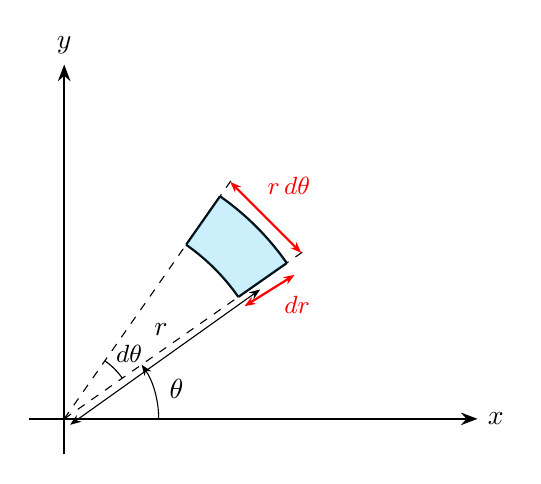
\begin{tikzpicture}[scale=1.5]

% Axes
\draw[-{Stealth[length=6pt]}, thick] (-0.3,0) -- (3.5,0) node[right] {$x$};
\draw[-{Stealth[length=6pt]}, thick] (0,-0.3) -- (0,3) node[above] {$y$};

% Radii
\draw[dashed, thin] (0,0) -- ({2.5*cos(35)},{2.5*sin(35)});
\draw[dashed, thin] (0,0) -- ({2.5*cos(55)},{2.5*sin(55)});

% Arcs
\draw[thick] ({1.8*cos(35)},{1.8*sin(35)}) arc (35:55:1.8);
\draw[thick] ({2.3*cos(35)},{2.3*sin(35)}) arc (35:55:2.3);

% Radial lines of element
\draw[thick] ({1.8*cos(35)},{1.8*sin(35)}) -- ({2.3*cos(35)},{2.3*sin(35)});
\draw[thick] ({1.8*cos(55)},{1.8*sin(55)}) -- ({2.3*cos(55)},{2.3*sin(55)});

% Fill area element
\fill[cyan, opacity=0.2]
  ({1.8*cos(35)},{1.8*sin(35)}) arc (35:55:1.8) --
  ({1.8*cos(55)},{1.8*sin(55)}) -- ({2.3*cos(55)},{2.3*sin(55)}) arc (55:35:2.3) --
  ({2.3*cos(35)},{2.3*sin(35)}) -- cycle;

% Labels for dr and r*dtheta
\draw[{Stealth[length=4pt]}-{Stealth[length=4pt]}, red, thick]
  ({2.45*cos(35)},{2.45*sin(35)}) -- ({2.45*cos(55)},{2.45*sin(55)});
\node[red, above right] at ({2.45*cos(48)},{2.45*sin(48)}) {\small $r\,d\theta$};

\draw[{Stealth[length=4pt]}-{Stealth[length=4pt]}, red, thick]
  ({1.8*cos(32)},{1.8*sin(32)}) -- ({2.3*cos(32)},{2.3*sin(32)});
\node[red, right] at ({2.1*cos(32)},{2.1*sin(32)-0.15}) {\small $dr$};

% r label
\draw[{Stealth[length=4pt]}-{Stealth[length=4pt]}, thin] (0.05,-0.05) -- ({2.05*cos(35)-0.02},{2.05*sin(35)-0.08});
\node[above] at ({1.0*cos(35)},{1.0*sin(35)+0.05}) {$r$};

% Angle
\draw[-{Stealth[length=4pt]}, thin] (0.8,0) arc (0:35:0.8);
\node at (0.95,0.25) {$\theta$};
\draw[thin] ({0.6*cos(35)},{0.6*sin(35)}) arc (35:55:0.6);
\node at (0.55,0.55) {\small $d\theta$};

\end{tikzpicture}
\end{document}
